As explained in Section \ref{v1.interface.requirement.section}, when drafting requirements for collecting the prompt-guided sketch text dataset, we iterated through several versions, and here we show the progression.
An excerpt from an old version of the instructions, in which we tried to explain a single \textit{step} of the annotation:
\begin{quotation}
In each task, we show \textbf{1 prompt} from which we would like to get
\begin{enumerate}
    \item A drawing containing 1 \textbf{entity} that you think illustrates the prompt.
    \item Text annotation for every \textbf{``component''} that makes up the entity.
    The word ``component'' is intentionally vague, and it depends on how you compose your drawing. For example, in the above example, the prompt is ``smiley face'', and during the process of creating a ``smiley face'' entity, we used 4 components: a face, a left eye, a right eye, and a mouth. For each component, you can annotate with ``face'', ``left eye'', ``right eye'', ``mouth'', respectively; you can also annotate with more details describing the shapes of each component: ``face that looks like an arc opening downwards'', ``a left eye that is an arc'', ``a right eye that looks exactly like the left eye'', ``an arc-like mouth''. Try to use creative and descriptive languages. You can draw a component using multiple strokes.
\end{enumerate}
\end{quotation}
% We also need to come up with examples explaining each requirement. 
% We select a few major sub-versions of the requirements resulted from circulating the interface within our lab.  

% Requirements and selected examples used in the first release in lab (Item 1 to 3 meant to enforce principal \ref{data_design_1}; Item 4 to 6 for \ref{data_design_2} and \ref{data_design_3}):
Requirements and selected examples used in the first version of the requirement:
\begin{enumerate}
\item Do not draw entity that does not respond to the prompt. For example, given the prompt \textit{Smiley Face}, the drawing should not contain irrelevant objects like a house. 
\item Do not draw more than one entity that responds to the prompt. For example, One should not draw two \textit{Smiley Face} entities, although each \textit{Smiley Face} entity is good. However, you can draw multiple tree objects to illustrate the prompt \textit{Forest}.  
\item \label{v1_requirement1_3} Do not draw entity that is ambiguous in terms of illustrating the prompt. For example, the drawing (Figure \ref{v1.requirement_1.1}) looks more like a \textit{Sad Face} than \textit{Smiley Face}.
\begin{figure*}[!h]
\centering

\includegraphics[width=.3\linewidth]{data_collection/host_amazon/hit_1/bad_smiley_face_ambiguous_face.png}
\caption{An example included in the first version of the requirements.}
\label{v1.requirement_1.1}
\end{figure*}

\item Do not draw one component that contains more information/content than what the annotation for that component describes. (A counterexample is illustrated in Figure \ref{v1.requirement_1.2}.)
\begin{figure*}[!h]
\centering
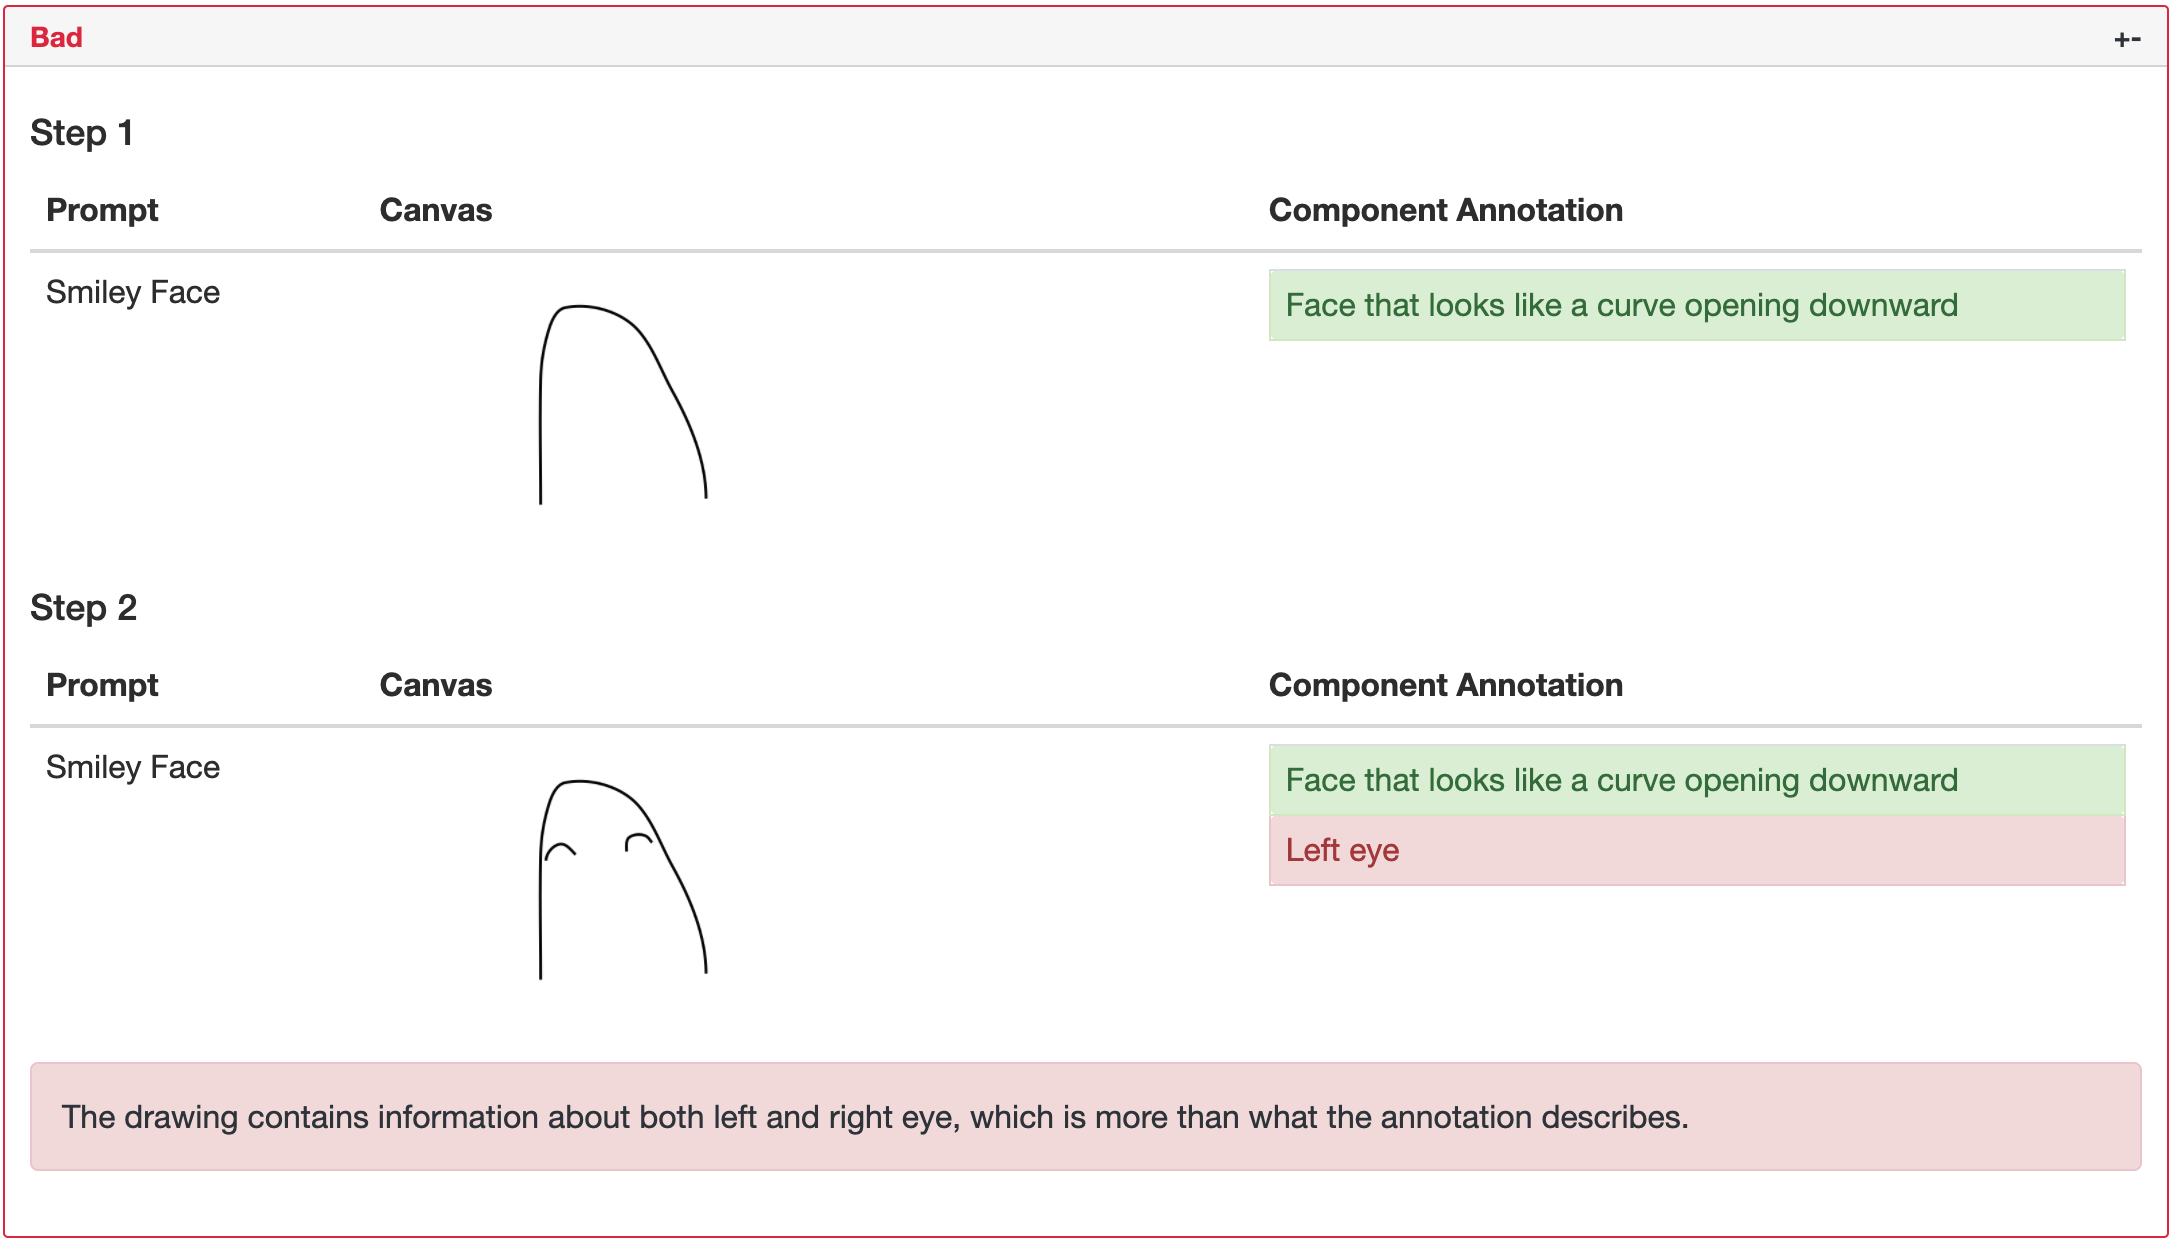
\includegraphics[width=.8\linewidth]{data_collection/v1_requirement1_bad1.png}  
\caption{An example of unaligned drawing and text description.}
\label{v1.requirement_1.2}
\end{figure*}

\item Do not split the drawing of a component into multiple steps, unless you can annotate each step separately. (A counterexample is illustrated in Figure \ref{v1.requirement_1.3}.)
\begin{figure*}[!h]
\centering
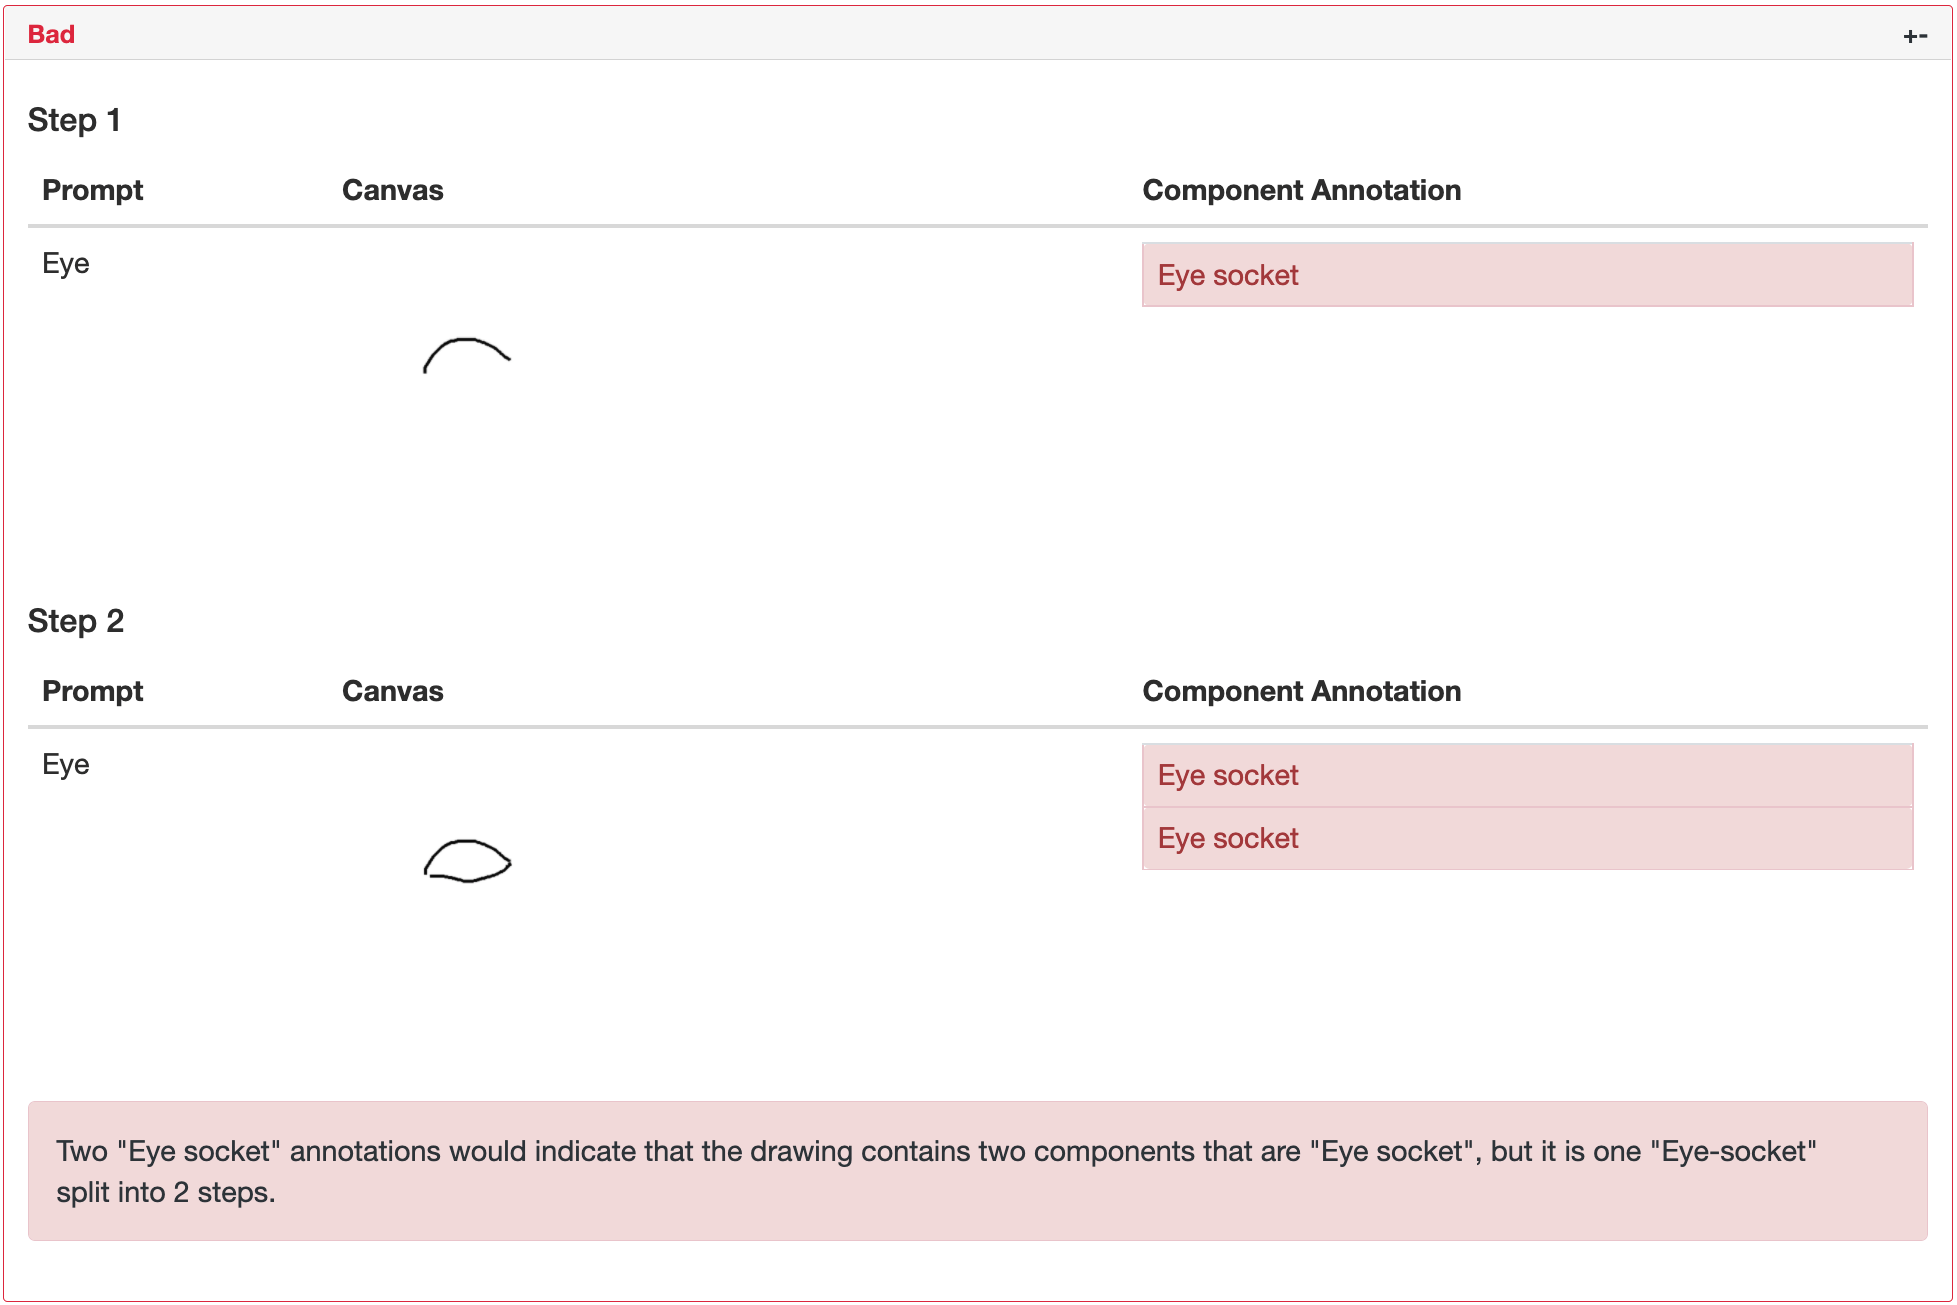
\includegraphics[width=.8\linewidth]{data_collection/v1_requirement1_bad2.png}  
\caption{An example of misalignment: text description \textit{overflow} into multiple steps.}
\label{v1.requirement_1.3}
\end{figure*}

\item Do not annotate a component more than once.
\end{enumerate}



% \begin{figure*}[!htb]
% % \ContinuedFloat
% \begin{subfigure}{\textwidth}
%     \centering
%     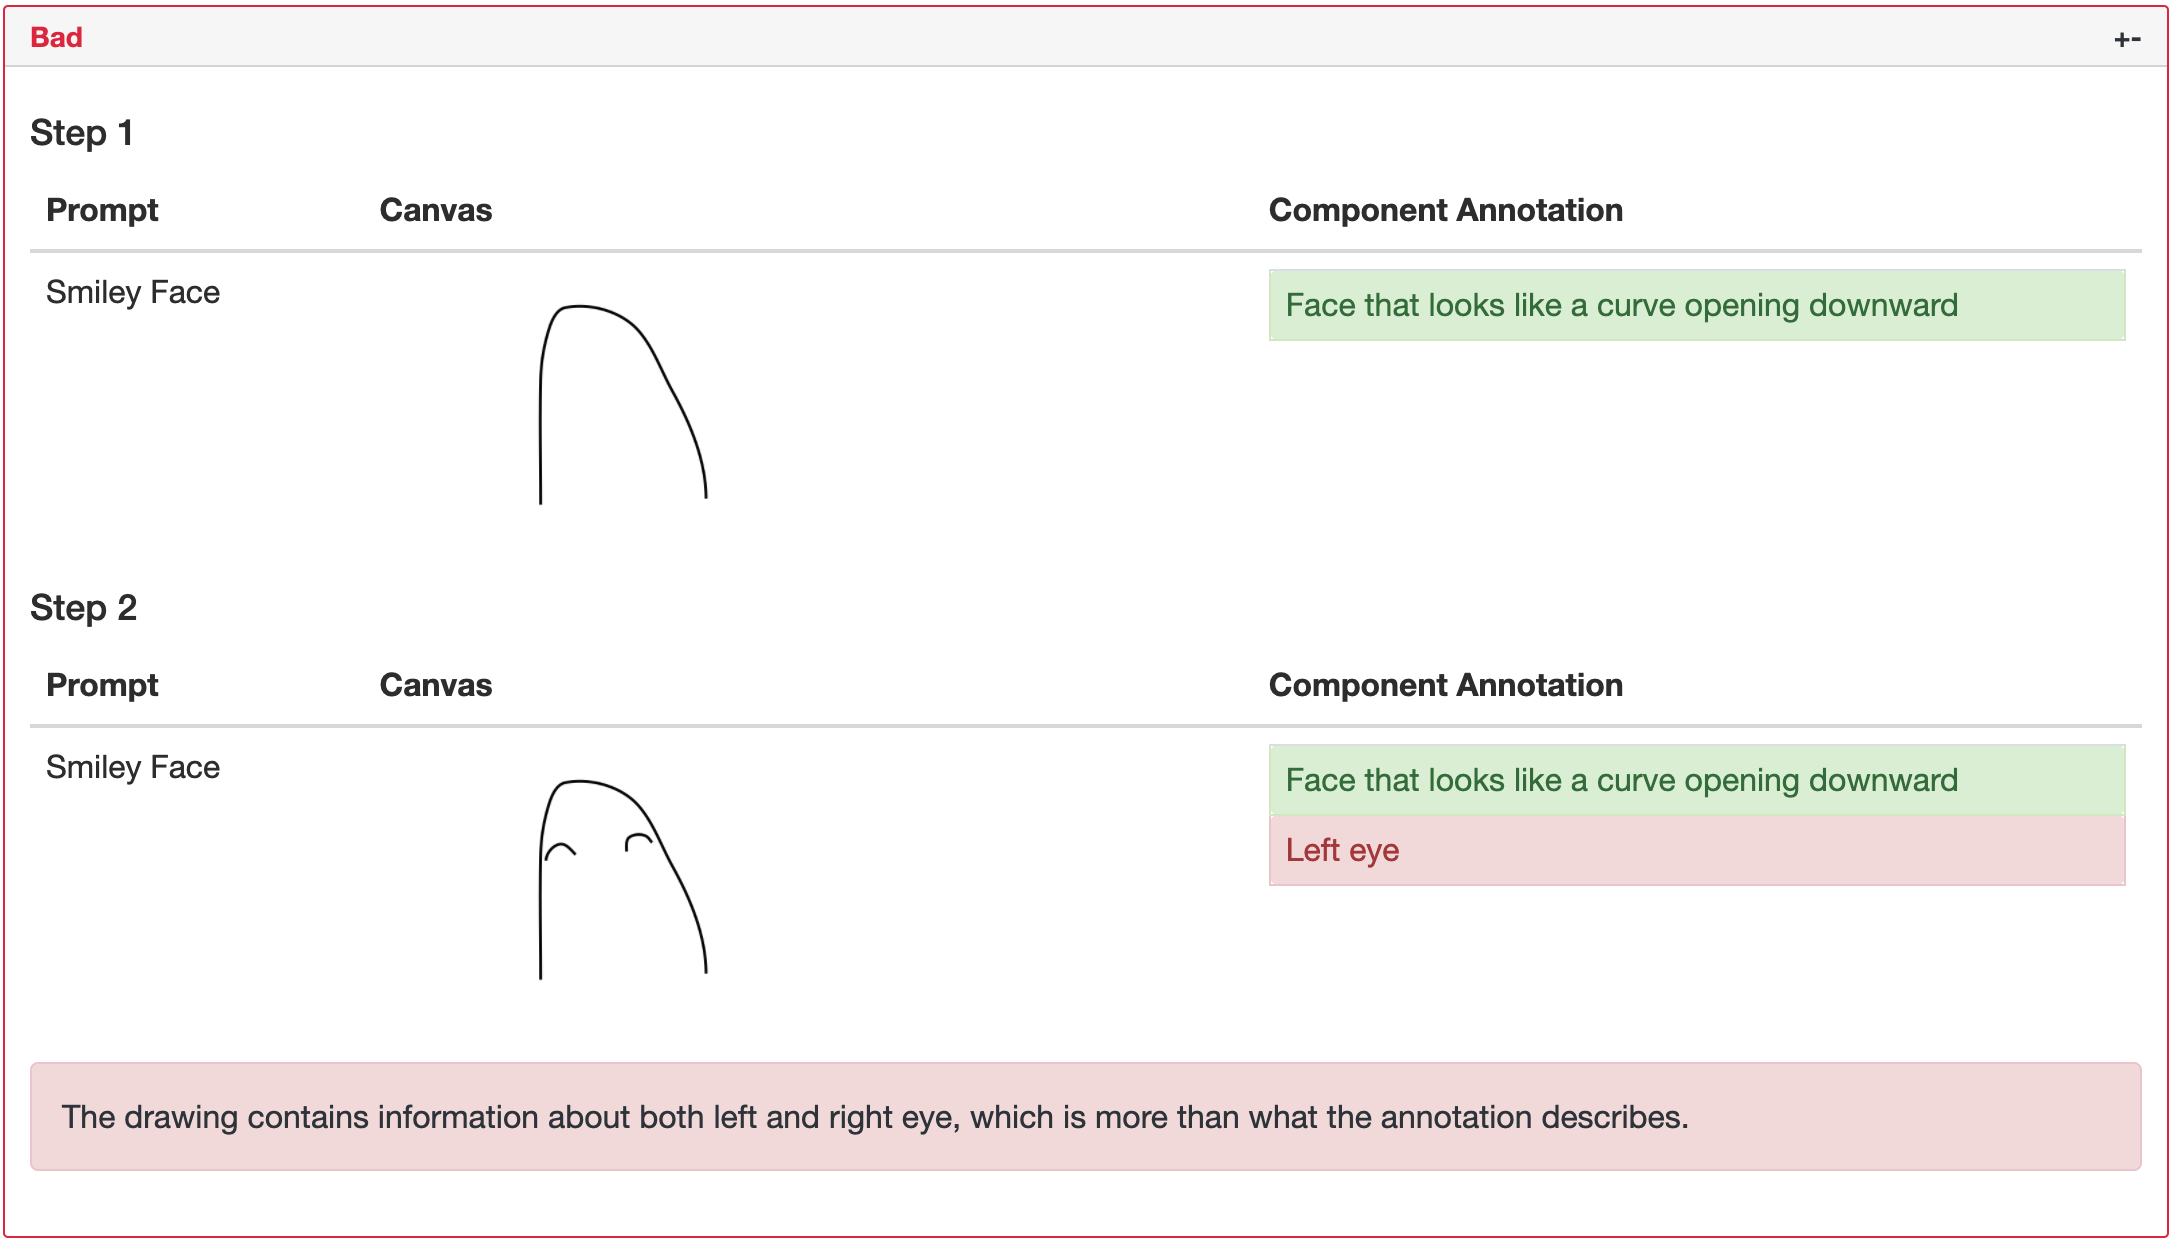
\includegraphics[width=.8\linewidth]{data_collection/v1_requirement1_bad1.png}  
%     \caption{Unaligned drawing and text description.}
%     \label{v1.requirement_1.2}
% \end{subfigure}
% \newline
% \begin{subfigure}{\textwidth}
%     \centering
%     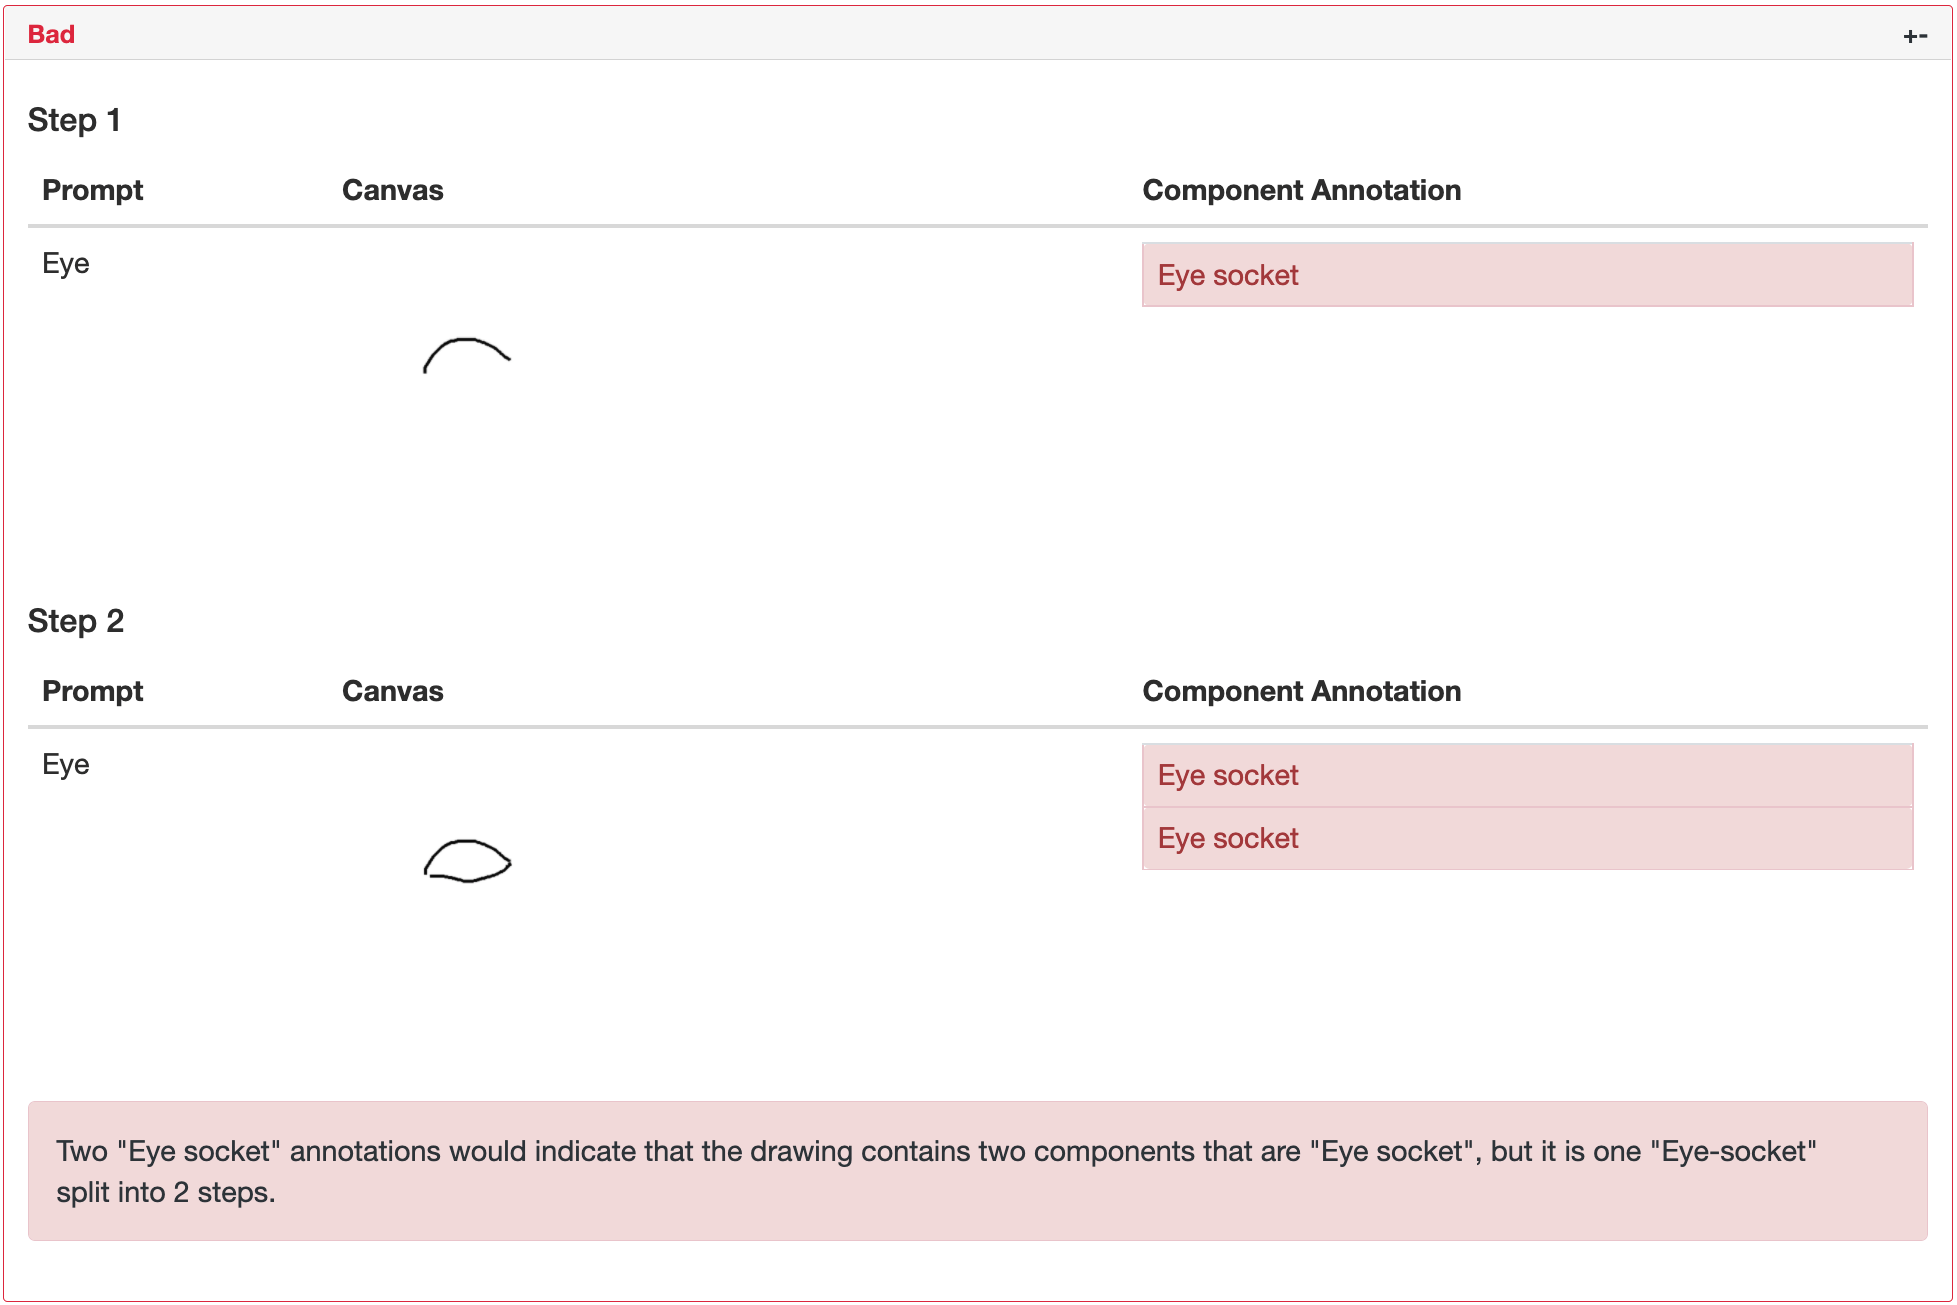
\includegraphics[width=.8\linewidth]{data_collection/v1_requirement1_bad2.png}  
%     \caption{An example of misalignment: text description \textit{overflow} into multiple steps.}
%     \label{v1.requirement_1.3}
% \end{subfigure}
% \caption{Counterexamples used in first version of the requirements in prompt-guided sketch text dataset.}
% \label{v1.requirement_1}
% \end{figure*}
% Figure 3x.a and 3x.b show some previous versions of the requirements. We eventually decided that  

% There is even more effort that went into defining the requirements of the task. This is really the section that we want to use to enforce all the DQ's. The final set of instructions is displayed in Figure x4.
% [Figure x4: final requirements]

% Comparing examples in requirements format:

% Methods to help understand the requirements. 
% Specifying which examples demonstrate which requirements, add next to the questions which requirement the question is testing. 

% Requirements and selected examples used in the second release in lab (Item 4 is meant to enforce principal \ref{data_design_1}; the other items for \ref{data_design_2} and \ref{data_design_3}):
Second version of the requirement section in text-guided sketch text dataset:
\begin{enumerate}
\item Draw \textit{one} item at a time and provide its corresponding annotation. For example, the text annotation says ``left eye'', but two items are drawn: a left eye and a right eye.
\item The annotation should describe its corresponding item in the drawing \textit{entirely}.
\item The annotation should name the item.
\item Desired properties of good drawings:
\begin{itemize}
    \item Contain as many items as possible, but be sure that they all contribute to illustrating the prompt. For example, draw more than just two eyes for a face.
    \item Use shapes creatively. For example, draw a triangle for the left eye, and annotate accordingly with ``triangular left eye that shows suspicion''.
\end{itemize}
\item Desired properties of good annotations:
\begin{itemize}
    \item Use descriptive languages. For example, ``a left eye that looks an arc facing downward''.
    \item Include the intention/purpose of drawing an item. Explain in the annotation reasons for drawing the item. For example, ``thumbs-up next to the face that really shows how happy the face is''.
\end{itemize}
\end{enumerate}

Third version of the requirement section in text-guided sketch text dataset:
\begin{enumerate}
\item Each drawing should contain at least 2 steps.
\item Annotation of each step should include at least the name of the drawn object(s).
\item If draw multiple copies of the same object, draw each object in a separate step and give different annotations by using, for example, cardinal or ordinal numbers. (An example shown in Figure \ref{v1.requirement_3})
\item Differentiate between plural and singular forms.
\item The name of the whole should not be used for its parts. (An example shown in Figure \ref{v1.requirement_3})
\begin{figure*}[!h]
\centering
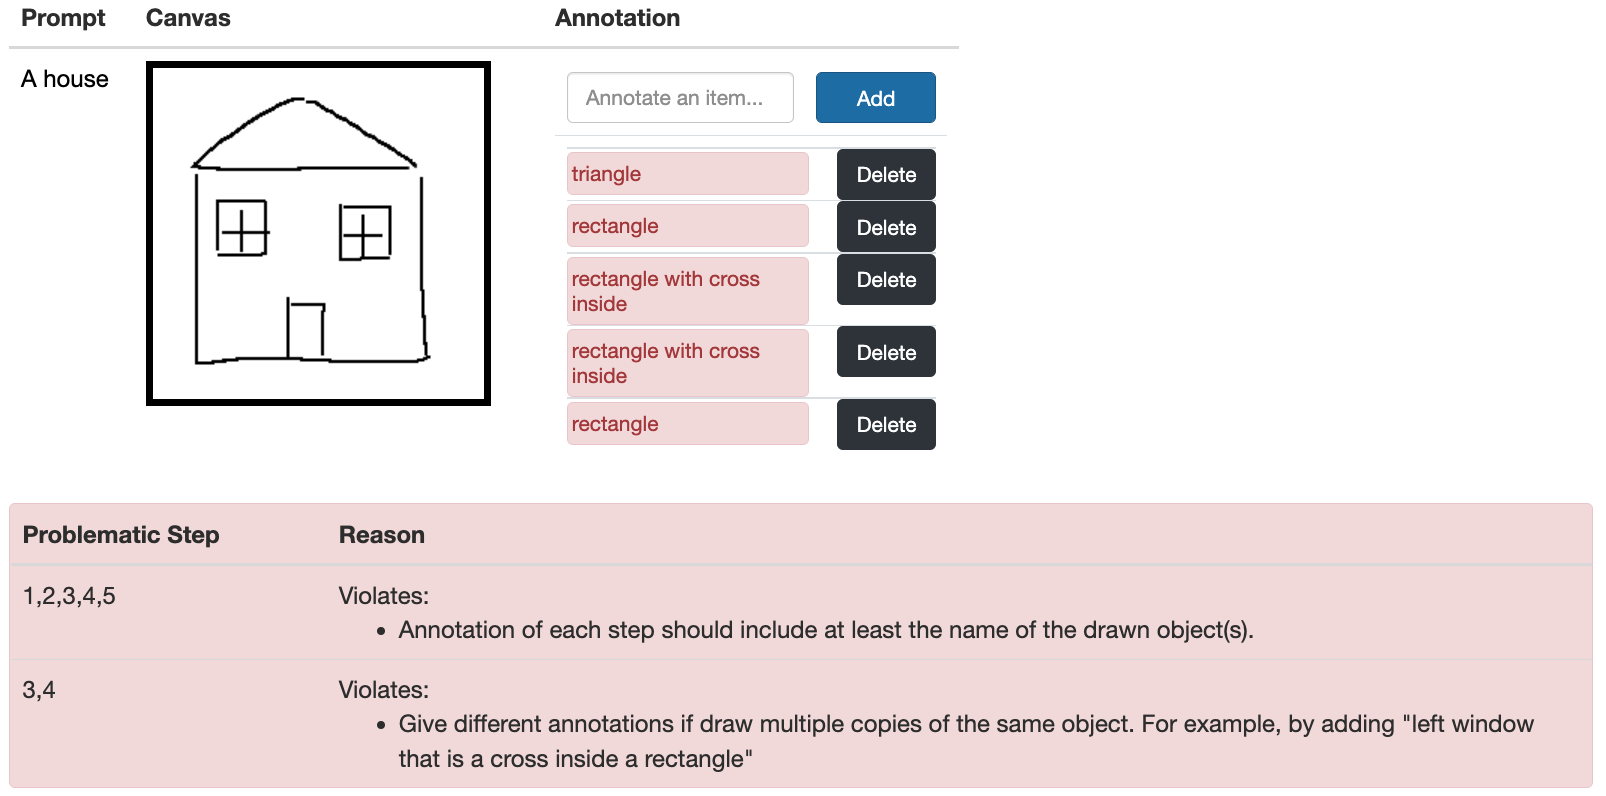
\includegraphics[width=.8\linewidth]{data_collection/v1_requirement3_bad1.png}  
\caption{A counterexample used in third version of the requirements.}
\label{v1.requirement_3}
\end{figure*}
    
\item The word "right" always refers to this side: $\Longrightarrow$
\end{enumerate}




